%%%%%%%%%%%%%%%%%%%%%%%%%%%%%%%%%%%%%%%%%
% Short Sectioned Assignment LaTeX Template Version 1.0 (5/5/12)
% This template has been downloaded from: http://www.LaTeXTemplates.com
% Original author:  Frits Wenneker (http://www.howtotex.com)
% License: CC BY-NC-SA 3.0 (http://creativecommons.org/licenses/by-nc-sa/3.0/)
%%%%%%%%%%%%%%%%%%%%%%%%%%%%%%%%%%%%%%%%%

%----------------------------------------------------------------------------------------
%	PACKAGES AND OTHER DOCUMENT CONFIGURATIONS
%----------------------------------------------------------------------------------------

\documentclass[paper=a4, fontsize=11pt]{scrartcl} % A4 paper and 11pt font size

% ---- Entrada y salida de texto -----

\usepackage[T1]{fontenc} % Use 8-bit encoding that has 256 glyphs
\usepackage[utf8]{inputenc}
%\usepackage{fourier} % Use the Adobe Utopia font for the document - comment this line to return to the LaTeX default

% ---- Idioma --------

\usepackage[spanish, es-tabla]{babel} % Selecciona el español para palabras introducidas automáticamente, p.ej. "septiembre" en la fecha y especifica que se use la palabra Tabla en vez de Cuadro

% ---- Otros paquetes ----

\usepackage{url} % ,href} %para incluir URLs e hipervínculos dentro del texto (aunque hay que instalar href)
\usepackage{amsmath,amsfonts,amsthm} % Math packages
%\usepackage{graphics,graphicx, floatrow} %para incluir imágenes y notas en las imágenes
\usepackage{graphics,graphicx, float} %para incluir imágenes y colocarlas

\usepackage{listings}	%para incluir remarcado para comandos bash

% Para hacer tablas comlejas
%\usepackage{multirow}
%\usepackage{threeparttable}

%\usepackage{sectsty} % Allows customizing section commands
%\allsectionsfont{\centering \normalfont\scshape} % Make all sections centered, the default font and small caps

\usepackage{fancyhdr} % Custom headers and footers
\pagestyle{fancyplain} % Makes all pages in the document conform to the custom headers and footers
\fancyhead{} % No page header - if you want one, create it in the same way as the footers below
\fancyfoot[L]{} % Empty left footer
\fancyfoot[C]{} % Empty center footer
\fancyfoot[R]{\thepage} % Page numbering for right footer
\renewcommand{\headrulewidth}{0pt} % Remove header underlines
\renewcommand{\footrulewidth}{0pt} % Remove footer underlines
\setlength{\headheight}{13.6pt} % Customize the height of the header

\numberwithin{equation}{section} % Number equations within sections (i.e. 1.1, 1.2, 2.1, 2.2 instead of 1, 2, 3, 4)
\numberwithin{figure}{section} % Number figures within sections (i.e. 1.1, 1.2, 2.1, 2.2 instead of 1, 2, 3, 4)
\numberwithin{table}{section} % Number tables within sections (i.e. 1.1, 1.2, 2.1, 2.2 instead of 1, 2, 3, 4)

\setlength\parindent{0pt} % Removes all indentation from paragraphs - comment this line for an assignment with lots of text

\newcommand{\horrule}[1]{\rule{\linewidth}{#1}} % Create horizontal rule command with 1 argument of height

\usepackage{booktabs}
\usepackage{tabularx}
\usepackage{multicol} 


%----------------------------------------------------------------------------------------
%	TÍTULO Y DATOS DEL ALUMNO
%----------------------------------------------------------------------------------------

\title{
\normalfont \normalsize 
\textsc{\textbf{Ingeniería del conocimiento (2020-2021)} \\ Máster en ingeniería informática \\ Universidad de Granada} \\ [25pt] % Your university, school and/or department name(s)
\horrule{0.5pt} \\[0.4cm] % Thin top horizontal rule
\huge Lógica difusa aplicada a los semáforos \\ % The assignment title
\horrule{2pt} \\[0.5cm] % Thick bottom horizontal rule
}
\author{Manuel Orantes Taboada, Carlos Sanchez Martinez} % Nombre y apellidos


\date{\normalsize\today} % Incluye la fecha actual

%----------------------------------------------------------------------------------------
% DOCUMENTO
%----------------------------------------------------------------------------------------

\begin{document}

\maketitle % Muestra el Título

\newpage %inserta un salto de página

\tableofcontents % para generar el índice de contenidos

\newpage

\section{Resumen}
Actualmente los semáforos de todo el mundo funcionan con ciclos fijos de tiempo predeterminado. Desde que se definieran los principios de lógica difusa, muchos han sido los trabajos que han enfocado este tema, y se han realizado aproximaciones con lógica difusa por todo el mundo. Uno de los principales trabajos fue el propuesto por Pappis y Mamdani, y muchos otros siguieron sus pasos a lo largo de los últimos años. La idea del funcionamiento del controlador es la siguiente: a partir de unas reglas que se han sacado a base de ensayo y error, se calcula el grado de confianza para clasificar el tiempo de retraso de los coches, siendo la llegada de estos aleatoria. Con todos estos datos se consigue minimizar el tiempo de espera de los vehículos. Hoy en día se siguen desarrollando tanto teorías como sistemas que en un futuro nos permitan vivir sin tantos atascos, consiguiendo a su ven reducir el tiempo de espera de los conductores, y la emisiones producidas por los mismos.

\textbf{Keywords: lógica difusa, cruce de carreteras , semáforo inteligente, controlador difuso} 

\section{Introducción}

La mayoría de las señales de tráfico de hoy en día están controladas por ciclos fijos de tiempo, es decir, el semáforo está en verde durante $x$ segundos y después está en rojo durante $y$ segundos, siendo normalmente distintos $x$ e $y$. Esto es una solución muy simple, pero que no suele ayudar en la congestión del tráfico, haciendo que esta no sea ni mucho menos la óptima. Pero ha habido muchos avances en la tecnología, y los semáforos inteligentes no deben de ser ignorados, sobre todo en las grandes urbes que mueven inmensas cantidades de tráfico. 

\section{Diferentes estudios sobre los controladores de semáforos con lógica difusa}
Desde que Zadeh(1921-2017) definiera en 1965 los conceptos de la lógica difusa, esta se ha usado en multitud de proyectos, sobre todo los relacionados con la ingeniería. Entre ellos, se han realizado muchos estudios de la aplicación de la lógica difusa a los semáforos.\\

El más popular fue el que propusieron Pappis y Mamdani \cite{Mamdani}. Construyeron un modelo para un cruce de dos vías en donde cada vía solo tenía un carril. Después, fueron sucesivos trabajos los que se fueron presentando, entre ellos destacaremos los de Nakatsuyama \cite{Nakatsuyama} o Favilla \cite{Favilla}, que ya introducían múltiples carriles en el modelo. Incluso en un trabajo de Trabia \cite{Trabia} se simuló un cruce con cuatro carriles, incluyendo la opción de que los coches giraran a la derecha en el cruce. Hay que especificar que, en este último paper, al igual que en otros como el de Pappis y Mamdani \cite{Mamdani}, se hizo el estudio en Reino Unido, y lo que se permitía es que los coches giraran a la izquierda, debido a que conducen en sentido opuesto a lo que estamos acostumbrados. Para facilitar la comprensión, se han unificado todos estos criterios tomando de referencia que se circula por la derecha, y por lo tanto, cambiamos el sentido de los papers realizados en Inglaterra.\\

Después, hubo otra vertiente de trabajos cuyo objetivo era minimizar el tiempo de espera, hasta obtener el óptimo. Ella Bingham \cite{Ella} usó la misma configuración que usaron Pappis y Mamdani \cite{Mamdani}. En su estudio, los parámetros que definía el controlador del semáforo de Mamdani fueron determinados mediante aprendizaje por refuerzo basado en simulaciones. En su trabajo, ella misma comentó que conseguía un gran resultado con volúmenes de tráfico constantes. Chou y Teng \cite{Chou} extendieron el controlador de las señales de tráfico para resolver el problema de varios cruces consecutivos. Su controlador podía ser usado hasta con colas de más de 700 metros. Disponían de diferentes sensores a lo largo del recorrido para obtener la información del tráfico. Usaban una ecuación parabólica, debido a su simplicidad, para simular el tránsito de los vehículos. Su objetivo era construir un simulador de tráfico que se asemejara al del mundo real. Usaban la longitud máxima de la cola de coches para las direcciones relativas de las intersecciones. Notar que en su trabajo usaron longitudes diferentes a las que se usaron en los primeros papers de los que hemos hablado.\\

Chong \cite{Chong} investigó los resultados de 4 redes neuronales difusas como arquitecturas distintas para un controlador de semáforo para un simple cruce de 4 direcciones. El entrenamiento de las redes neuronales difusas fue realizado con datos recogidos de un simulador de tráfico por un operario que sí era humano.
Indicó que todas las arquitecturas probadas realizaban un buen trabajo. Schmöcker \cite{Scho} en cambio realizó un estudio en el que prestó un especial interés en la espera de los peatones en los cruces de cuatro direcciones.\\

Como podemos observar, son muchos los estudios que se han realizado en este campo, con multitud de configuraciones. Los cambios más comunes siempre han sido tener en cuenta uno o más cruces o la cantidad de carriles de estos. También, como hemos visto, se han tenido en cuenta a los peatones o si en el cruce se podía girar a la derecha o no. Además, se han probado multitud de técnicas diferentes, aunque todas tienen como base a la lógica difusa. 

\newpage
Lo que sí tienen todos en común, es que para realizar el estudio se ha creado un simulador de tráfico para poder tener una referencia de cómo se están comportando los controladores de los semáforos en un ambiente preparado para asemejarse lo más posible a la realidad. Veamos ahora un ejemplo de como podría funcionar un simulador de tráfico para un cruce como el siguiente:

\begin{figure}[H]
	\centering
	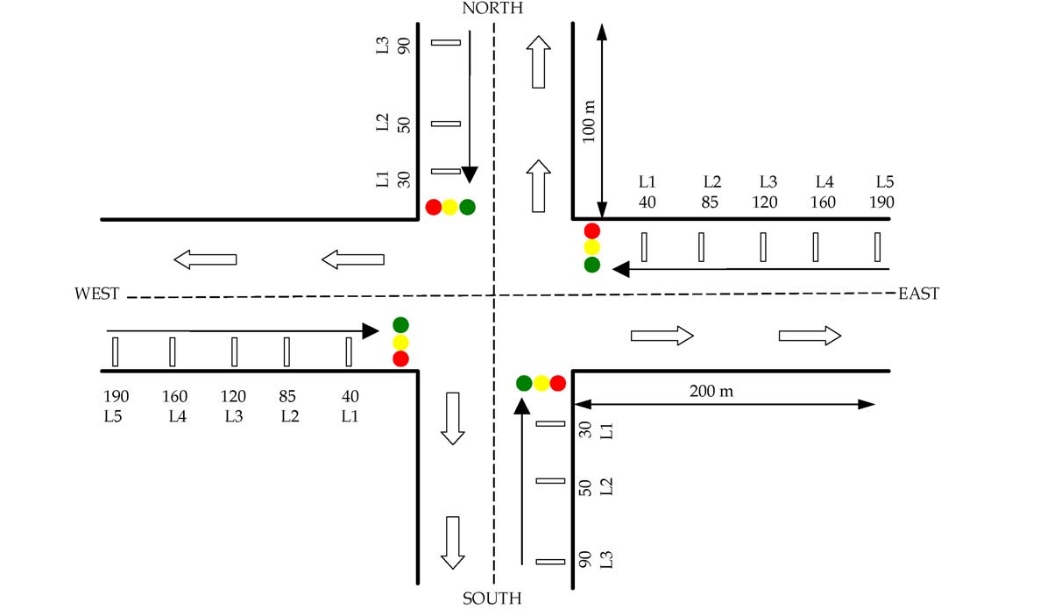
\includegraphics[width=1\linewidth]{cruce1}

	\label{fig:cruce1}
\end{figure}

\newpage

\section{Otros trabajos relacionados}
Como acabamos de ver, en los trabajos se estudia como mejorar la eficacia de los ciclos de los semáforos a partir de un flujo de tráfico, que casi siempre es proporcionado por distintos simuladores de tráfico. Pero hay algunos estudios que también usan lógica difusa que se encargan de eso mismo, de calcular si hay congestión de tráfico o no. Este es el caso de un reciente estudio de Kalinic \cite{California} (2019). En el se busca justo eso, ver por medio de técnicas difusas el estado de una de las carreteras de Estados Unidos, más concretamente de la interestatal 880, de California.

\begin{multicols}{2}

\begin{figure}[H]
	\centering
	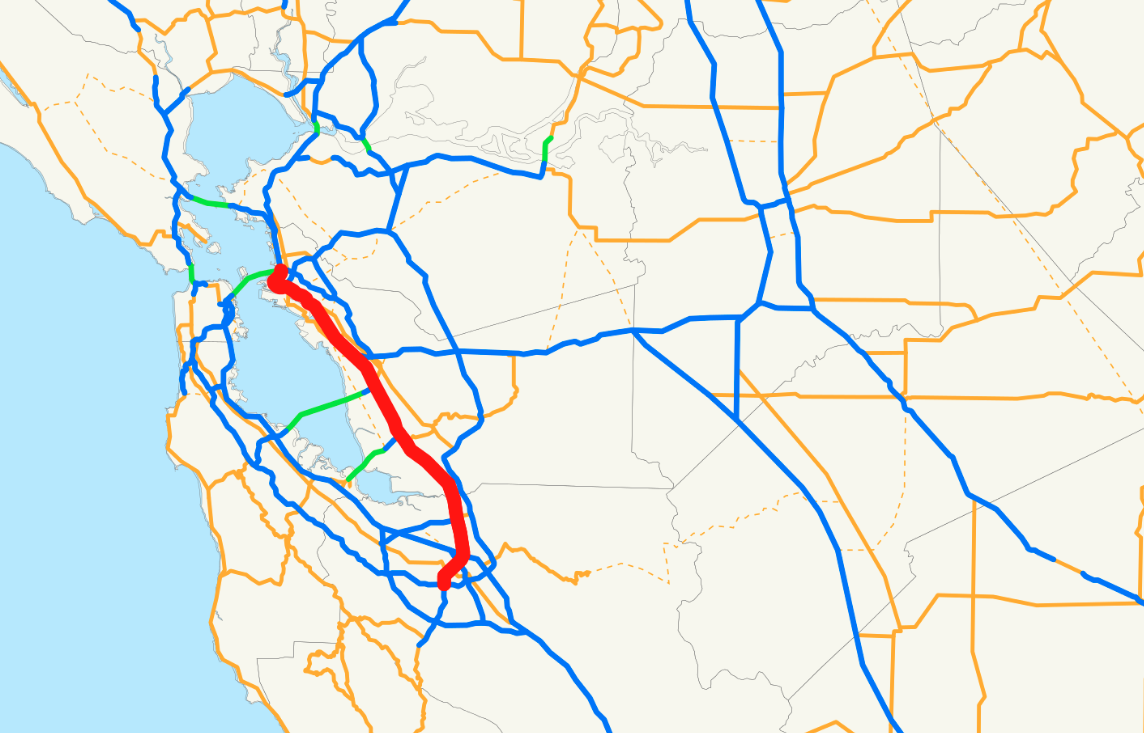
\includegraphics[width=1\linewidth]{interestatal}
	\label{fig:interestatal}
\end{figure}
\begin{figure}[H]
	\centering
	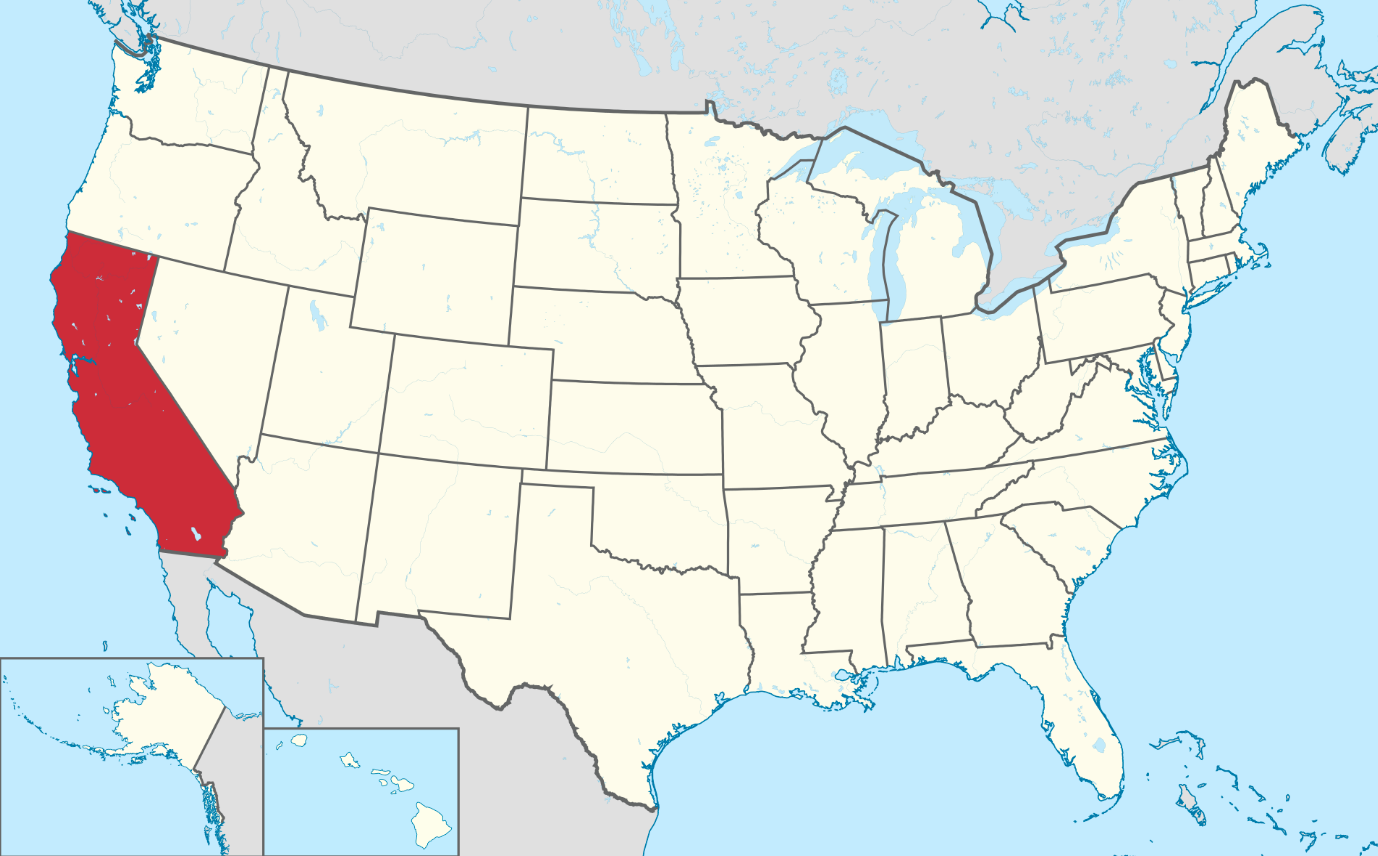
\includegraphics[width=1\linewidth]{california}
	\label{fig:california}
\end{figure}

\end{multicols}


\begin{multicols}{2}
	En el trabajo se dividía la carretera en 6 trozos, y se usaban los siguientes conjuntos difusos:
	\begin{itemize}
		\item Completamente libre de circulación.
		\item Libre de circulación.
		\item Circulación estable.
		\item Circulación inestable.
		\item Circulación cerca de congestionarse.
		\item Circulación congestionada.
		\item Circulación extremadamente congestionada.
	\end{itemize}
\begin{figure}[H]
	\centering
	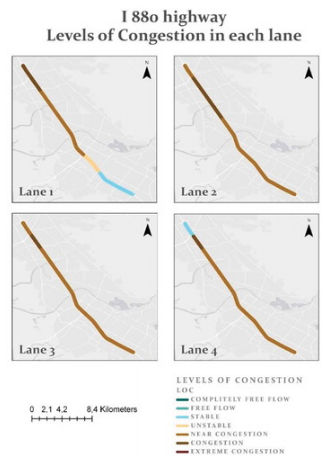
\includegraphics[width=1\linewidth]{set}
	\label{fig:set}
\end{figure}
\end{multicols}

En las conclusiones a las que llegaron, destacamos que se diferenciaban de los métodos clásicos de cálculo de congestión de carreteras, que ellos no usaban el número de coches en relación a un determinado segmento de la carretera. En cambio, su aproximación estaba basada en el lenguaje natural y el sentimiento de los conductores implicados en cada sector. Además, declaran que su método es sencillo de aplicar y sigue la lógica del sentido común, y que en un futuro le añadirían nuevas reglas referentes a la velocidad de los vehículos.

\section{Diseño de un simulador de tráfico para un cruce}
Vamos a ilustrar que sería necesario para la creación de un simulador de tráfico, usando unos datos ya dados según la anterior imagen. Para ello, los principales puntos que se deben de tener en cuenta son los siguientes:
\begin{itemize}
	\item La velocidad media que se da de una dirección a otra cuando el semáforo está en verde. En nuestro caso, tomaremos la velocidad media de los coches que van de oeste a este como 12 m/s.
	\item El tiempo necesario para alcanzar el semáforo desde los 200 metros en donde están situados los detectores. Asumiendo que no habrá ningún coche en cola, podemos hallar este tiempo usando la siguiente fórmula:
	$$ t = \frac{\Delta x}{v} = \frac{200m}{12m/s} = 16.66 s$$
	\item De manera similar situamos en 12m/s la velocidad media de un vehículo que circula de norte a sur y sabemos que tardará 8.33 segundos en recorrer los 100 metros que separan al semáforo de los sensores.
\end{itemize}

Es muy importante remarcar que la distancia de los sensores a los semáforos serán muy importantes a la hora de determinar el mínimo de la duración de un semáforo con estado abierto, es decir, con la luz verde. La duración del semáforo abierto o cerrado (es decir, en verde o en rojo) debe de modificarse teniendo en cuenta la cantidad de coches en cola en cada momento, paras intentar minimizar el tiempo que los coches esperar para cruzar. Por ejemplo, si tenemos una duración de un semáforo abierto de entre 20 y 120 segundos, cuando no haya ningún coche para pasar y en la otra dirección varios coches estén guardando cola, el semáforo deberá cerrarse para dejar pasar a los coches de la otra dirección. Además, debe de haber un valor máximo también sobre el cuál no pueda exceder el tiempo que un semáforo está abierto.\\

En los semáforos convencionales, la longitud de los vehículos no suele ser tenida en cuenta a la hora de ver la duración de las fases de los semáforos. A pesar de esto, la longitud real de los vehículos (que oscila desde los 4 metros hasta los 8) si es tomada en algunos estudios, como es el caso del paper de Chou y Teng \cite{Chou}. En otros estudios, los sensores han sido también utilizados para calcular el número de vehículos en cada carril y saber también la longitud de los vehículos aplicados, para dar una respuesta acorde de los estados de los semáforos.\\

Con todo esto, presentamos en la siguiente imagen como interactuarán cada una de las partes implicadas. Existen 4 generadores de vehículos, uno en cada dirección, que confluyen en el cruce, el cual está controlado por el simulador del semáforo.

\begin{figure}[H]
	\centering
	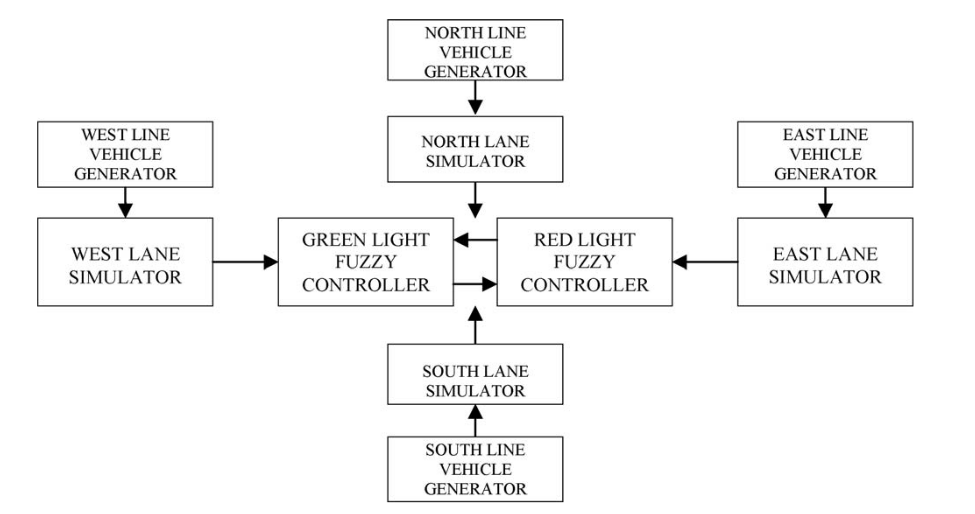
\includegraphics[width=1\linewidth]{cruce2}

	\label{fig:cruce2}
\end{figure}


En la realidad, los datos reales pueden adquirirse poniendo diferentes detectores en los carriles próximos a la intersección, en intervalos propicios. Si estos datos son imposibles de obtener por la fisionomía de la intersección, o por el presupuesto escaso, debemos de poder obtener datos que se muestren lo más reales posible, mediante lectores de flujo del tráfico. Por esto es tan importante la creación de un sistema de simulación de tráfico adecuado a nuestro problema.


\section{Modelo}

En este apartado describiremos el modelos que se va a usar para resolver el problema con lógica difusa.\\

En primer lugar la llegada de vehículos va a ser aleatoria. El proceso de selección estará dividido en 2 ciclos, el ciclo de luz roja y el ciclo de luz verde. El proceso asume que tienen una duración de 10 s/ciclo. Los vehículos dejan la cola en un ratio constante que llamaremos saturación que va a tener el valor de $3600$ vehículos/h en ambos brazos del cruce.
\newpage
Tenemos que si el vehículo llega como valor 1 y 0 si el vehículo no llega. Por lo que tenemos:

$$ q_n = \begin{cases} 1, & \mbox{si el vehículo llega durante un intervalo } n \\ 0, & \mbox{si el vehículo no llega } \end{cases} $$


Tenemos que $Q_G$ es el numero de vehículos que no han pasado en el estado de luz verde. Por lo que el número de vehículos totales en el intervalo $n$ del modelo se da de la siguiente manera:

$$Q_n=Q_G+=\sum_{i=1}^{n}q_i$$

El tiempo de espera de los vehículos viene dado por $D_{n,R}$ donde:\\

$$D_{n,R}=\sum_{i=1}^{n}(Q_G+=\sum_{j=1}^{i})$$

Tenemos $s$ como el flujo de saturación del cruce de los vehículos durante la fase de luz verde. Al comienzo de la fase de la luz verde tenemos que el número de vehículos no autorizados viene representado por $S_n$ donde $S_n$ es:\\

$$S_n=z*(Q_R+=\sum_{i=1}^{n}q_i-s*n)$$

Donde $Q_R$ es la cola que se formo durante el periodo rojo anterior y 

$$ z = \begin{cases} 1, & \mbox{Cuando multiplica por una cantidad no negativa} \\ 0, & \mbox{en otro caso } \end{cases} $$

Estos vehículos han sufrido un retraso de:

$$D_{n,G}=\sum_{i=1}^{n}z*(Q_R+=\sum_{j=1}^{i}q_j-s*i)$$

Durante un ciclo el tiempo total de retraso viene dado por:

$$D=D_{R,R}+D_{G,G}$$

y la media de retraso por vehículo será:

$$d_m=\frac{D}{\sum_{i=1}^{R+G}q_n}$$

Esta media de retraso sera comparada con la media obtenida con la siguiente fórmula, la media anterior será la que use nuestro sistema:

$$d_t=\frac{C(1-\lambda)}{2(1-\lambda*X)}+\frac{X^2}{2_q(1-X)}-0.65(\frac{C}{q^2})^{\frac{1}{3}}X^{2+5\lambda}$$

Para nuestro estudio usamos la media calculada como $d_m$ y mas tarde se comparará con el modelo que se construirá de lógica difusa. Una comparación de las dos medias calculadas se puede ver en la siguiente imagen.

\begin{figure}[H]
	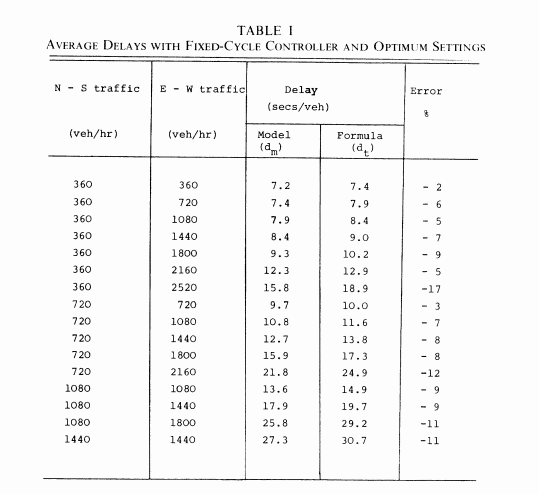
\includegraphics[scale=0.75]{tabla1}
	\centering
	\caption{Tabla de comparación de medias calculadas.}
	\label{fig:mesh1}
\end{figure}

En la tabla podemos ver la media calculada que es la que usa nuestro estudio y la media esperada que es la comparación, estas medias se usarán para comparar con el modelo de lógica difusa que veremos después.\\

\newpage
\section{Modelo de lógica difusa}

El modelo de lógica difusa que se va a usar usa una interpretación cuantitativa, con 4 variables, estas variables son:\\

T=\textit{variable tiempo que se le asigna los valores: "very short", "short", "medium", "long" y "very long"}.\\

A=\textit{Describe el número de vehículos que llegan a un brazo del cruce, puede tomar los valores: "none", "{a few}", "few", "many", "too many", "medium", "more than none", "more than a few", "more than few", "more than medium", "more than many", "more than too many"}.\\

Q=\textit{Describe los vehículos que hay en cola, puede tomar los valores: "{any}", "less than very small", "less than small", "less than small plus", "less than medium", "less than long" y "less than very long"}.\\

E=\textit{Variable Extensión, tiene el mismo valor que T}.\\

Para tomar decisiones se usarán instrucciones de la forma:
\begin{lstlisting}
if T = medium and A = mt(medium) and Q = lt(small)
	then E = medium
else
	if T = long and A = mt(many) and Q = lt(medium)
		then E = long
\end{lstlisting}

Donde los operadores and y else son operadores de \textbf{mínimo} y \textbf{máximo}.
En la frase P definida en $T \times A \times Q$,
\begin{lstlisting}
	if T= medium and A = mt(medium) and Q = lt(small)
\end{lstlisting}

Tenemos que $P=min\{\mu_{medium}(T),\mu_{mt(medium)}(A),\mu_{lt(small)}(Q)\}$
Donde $\mu_{medium}(T)$=grado de confianza de T, $\mu_{mt(medium)}(A)=$ grado de confianza de A y $\mu_{lt(small)}(Q)=$ grado de confianza de Q.
Y P=$\mu_p(T,A,Q)$.

Tenemos:
\begin{lstlisting}
if T= medium and A = mt(medium) and Q = lt(small)
	then E = medium
else
	if T= long and A = mt(many) and Q = lt(medium)
		then E = long
\end{lstlisting}

Donde la frase anterior formada por las instrucciones vista anteriormente se resuelve de la siguiente manera.

$$max\{min\{\mu_{medium}(T),\mu_{mt(medium)}(A),\mu_{lt(small)}(Q)\},min\{\mu_{long}(T),\mu_{mt(many)}(A),\mu_{lt(medium)}(Q)\}\}$$

Para obtener el grado de confianza de las distintas variables tenemos que mirar en las tablas que se muestran a continuación:

\begin{figure}[H]
	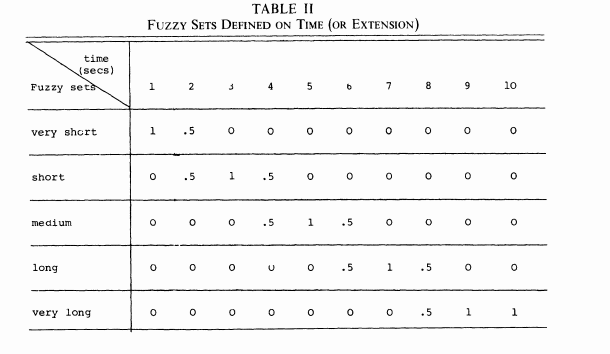
\includegraphics[scale=1]{tableTime}
	\centering
	\caption{Tabla de tiempo y Extensión.}

\end{figure}

\begin{figure}[H]
	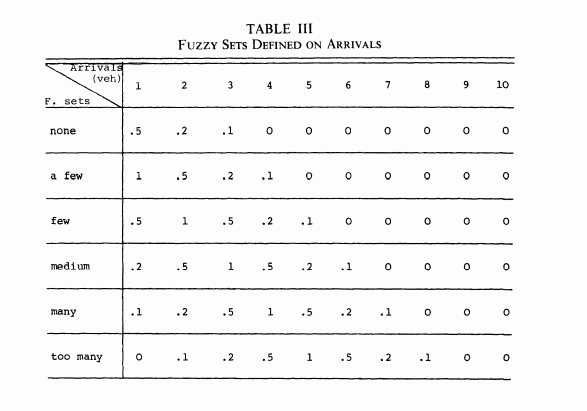
\includegraphics[scale=1]{tableArrivals}
	\centering
	\caption{Tabla de coches que llegan.}

\end{figure}

\begin{figure}[H]
	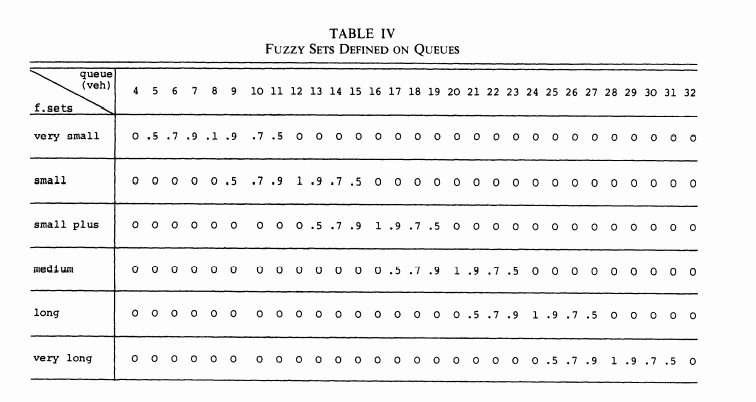
\includegraphics[scale=1]{tableQueues}
	\centering
	\caption{Tabla de coches en cola.}

\end{figure}

\begin{figure}[H]
	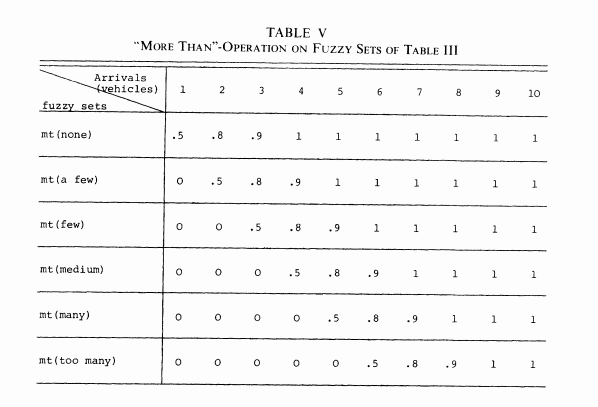
\includegraphics[scale=1]{tableMoreThan}
	\centering
	\caption{Tabla de more than.}

\end{figure}

\begin{figure}[H]
	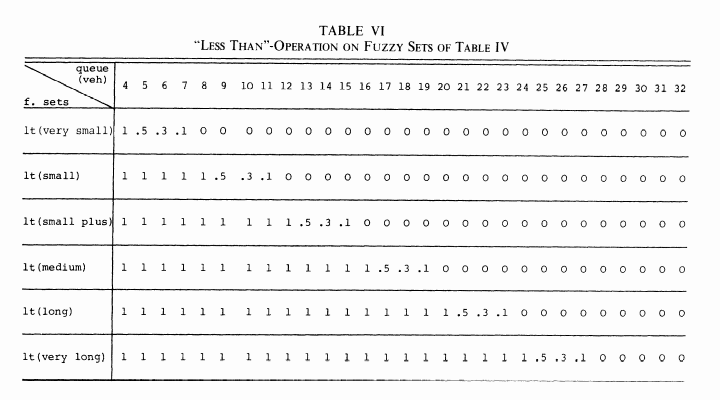
\includegraphics[scale=1]{tableLessThan}
	\centering
	\caption{Tabla de less than.}

\end{figure}

La descripción del proceso para decidir las acciones que se aplican vienen dadas como sigue.

Consideramos como el brazo correcto el brazo N-S del cruce y hay en cola por ejemplo 5 coches en el brazo E-O. Si tomamos un tiempo de 10s para el rango de tiempo de acción, creamos un vector con 10 posiciones cada una perteneciente a un segundo del tiempo dentro del rango de os 10s. en cada segundo tenemos el numero de vehículos que nos llega al brazo de cruce N-S. Por lo que nos queda un vector:

$$(0, 1, 0, 1, 1, 1, 1, 0, 0, 1)$$
Para el brazo E-O tenemos que:

$$(0, 1, 0, 0, 1, 0, 0, 1, 0, 0)$$

Desde estos vectores construimos otros donde ponemos las suma acumulada en cada segundo de los coches que han llegado en el instante de tiempo correspondiente, por lo que tenemos que para N-S:

$$(0, 1, 1, 2, 3, 4, 5, 5, 5, 6)$$

Y para el brazo E-O añadimos a la suma acumulativa en cada segundo los coches que tenemos en cola para ese brazo que eran 5, entonces tenemos que:

$$(5, 6, 6, 6, 7, 7, 7, 8, 8, 8)$$

Podemos ver entonces que para el segundo 1 del brazo N-S no llega ningún coche y para el brazo E-O tenemos 5 que son los que hay en cola.\\

Para el segundo 4 tenemos que para el brazo N-S han llegado hasta ese momento 2 coches y para el brazo E-O tenemos que hay 6 coches uno que ha llegado nuevo hasta ese momento y los 5 que había en cola.\\

Con estos datos podemos empezar a poner valores a nuestras variables para ver el grado de confianza de estos valores y poder resolver nuestras reglas.\\

Aplicaremos una regla para cada instante de tiempo de los vectores visto antes y aplicando los valores que se ajusten a nuestro estudio, en este caso vamos a poner unos valores de ejemplo . De forma que para el segundo 1 tenemos que:

$$t=1, a=0, q=5, e=1$$

Donde:
$(t,a,q,e)=(1,0,5,1)=min\{\mu_{very short}(1), \mu_{mt(none)}(a), \mu_{any}(q)\}$ el grado de confianza de e es igual que el de t por lo que no lo ponemos, valor de any se coge el mínimo valor de todos los valores posibles para la columna 5 en la tabla queue.
Por lo que tenemos que:

$$(1,0,5,1)=min\{1, 0.5, 0\}$$

Para conseguir estos valores miramos en sus tablas respectivas, para el valor de t miramos en la tabla e tiempo, para el valor de a miramos en la tabla de coches que llegan y para el valor de q miramos en la tabla de coches en cola. Los valores t=1, a=0, q=5 son el numero de la columna que hay que mirar en cada tabla, t= igual al segundo correspondiente, a=a los coches llegados hasta ese segundo para el brazo N-S, q=Los coches en cola para el brazo E-O. Las filas vienen dados por los valores "very short" para t, "mt(none)" para a, y "any" para q.\\
Los valores encontrados en las tablas son los grados de confianza, después se selecciona el mínimo de los grados de confianza.\\
Para este ejemplo el mínimo del grado de confianza es 0.\\

En este estudio se usaron 5 reglas en 5 intervalos de tiempo distintos, las reglas que se usaron fueron:\\
\newpage
\begin{multicols}{2}
\begin{figure}[H]
	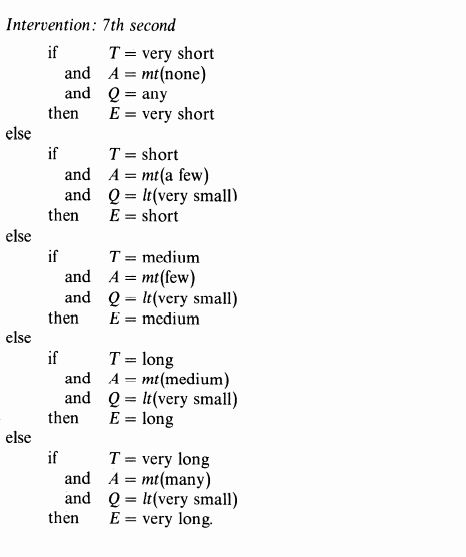
\includegraphics[scale=1]{reglas1}
	\centering
	\caption{Reglas 1.}
	
\end{figure}

\begin{figure}[H]
	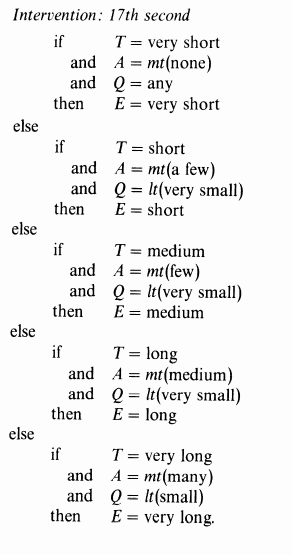
\includegraphics[scale=1]{reglas2}
	\centering
	\caption{Reglas 2.}
	
\end{figure}
\end{multicols}
\newpage
\begin{multicols}{2}
\begin{figure}[H]
	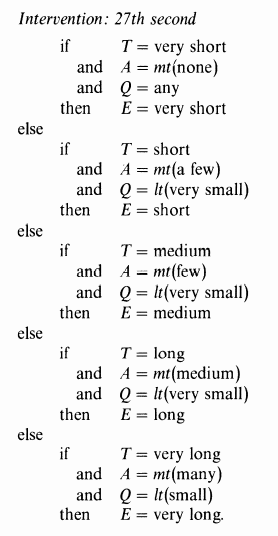
\includegraphics[scale=1]{reglas3}
	\centering
	\caption{Reglas 3.}

\end{figure}

\begin{figure}[H]
	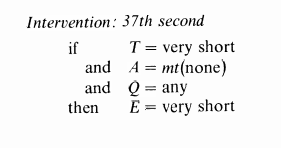
\includegraphics[scale=1]{reglas4}
	\centering
	\caption{Reglas 4.}

\end{figure}

\begin{figure}[H]
	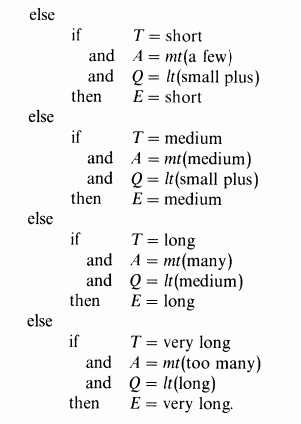
\includegraphics[scale=1]{reglas5}
	\centering
	\caption{Reglas 5.}


\end{figure}
\end{multicols}
 
\newpage



\begin{figure}[H]
	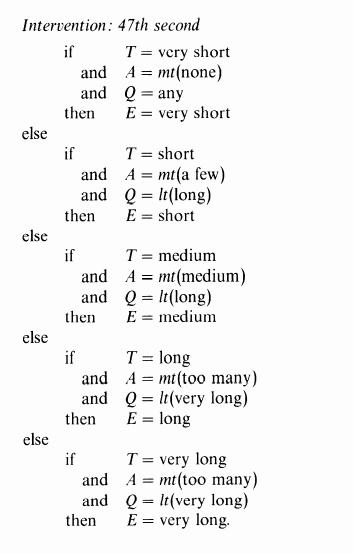
\includegraphics[scale=0.9]{reglas6}
	\centering
	\caption{Reglas 6.}

\end{figure}

Con estas reglas y usando el modelo de lógica difusa visto en este apartado, se ha comparado los resultados obtenidos con el modelo visto en el apartado anterior y los resultados fueron:\\

\begin{figure}[H]
	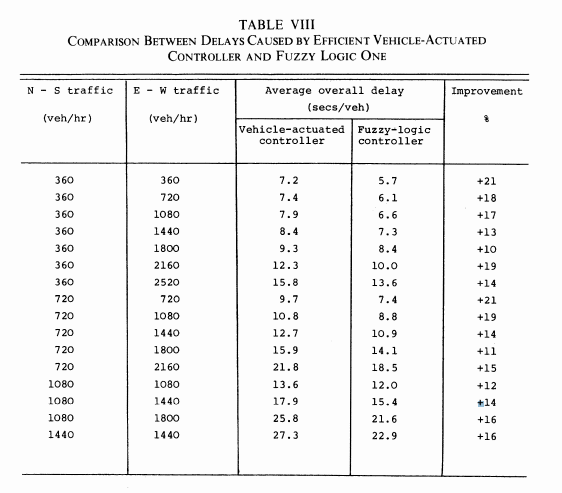
\includegraphics[scale=0.9]{resultados}
	\centering
	\caption{Resultados.}
\end{figure}


Podemos ver que en los resultados obtenidos se obtuvieron mejoras sustanciales al usar el controlador de lógica difusa. Aunque los resultados del controlador de lógica difusa fueron mejores que los del modelo del controlador anterior, en el estudio del modelo de lógica difusa, se han probado las reglas por ensayo y error por lo que se pueden mejorar los resultados obtenidos mediante un controlador de lógica difusa.\\

\newpage

\section{Uso de los semáforos inteligentes alrededor del mundo}

Está claro que hay decenas y decenas de papers sobre el tema que tratamos, pero, ¿se han llegado a usar estas técnicas en casos reales?

\subsection{Pittsburg, Pennsylvania (USA)}
''Todos conocemos los atascos. Causan estrés, pérdida de dinero y tiempo y una emisión extra de dióxido de carbono''. Así empieza artículo de Smart City Hub \cite{smart}. En el, se muestra el caso de Pittsburg, una ciudad de Pennsylvania, situada en Estados Unidos.\\

 Dicha ciudad ha conseguido reducir este terrible problema en un 40\%, debido, entre otras cosas, a la ayuda de los semáforos inteligentes. Como podemos ver, usan la tecnología Surtrac \cite{surtrac}. Indagando un poco más en la implementación de esta tecnología \cite{implementacion}, la compañía Rapid Flow usa tanto controladores de semáforos como cámaras para la detección de los vehículos, como podemos ver en la siguiente imagen:
\begin{figure}[H]
	\centering
	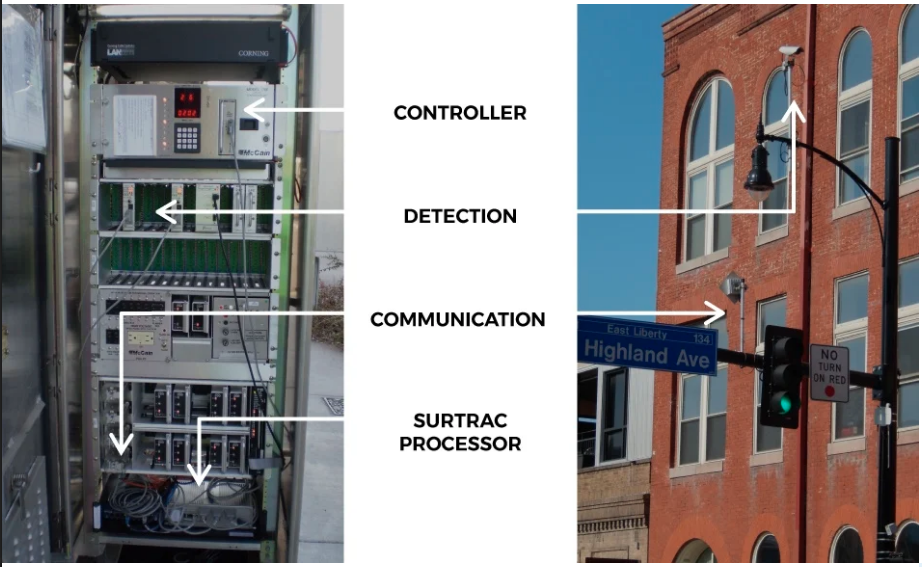
\includegraphics[width=1\linewidth]{surtrac}
	\label{fig:surtrac}
\end{figure}

Para ser más exactos, no he encontrado referencia a la utilización de lógica difusa, pero tampoco a la no utilización de la misma. Al fin y al cabo es un producto de esta compañía, y le conviene no enseñar todas sus cartas a la competencia. Lo más probable es que usen lógica difusa para el comportamiento de sus controladores.

\subsection{Artículo en MESinsights}

Podemos encontrar actualmente, que el los semáforos inteligentes están a la orden del día. Podemos ver como 
Cate Lawrence y Nicole Kareta hablan en su artículo \cite{MES} (2020) de cómo puede ayudar el uso de estos a las poblaciones, reduciendo los tiempos de espera de conductores y peatones.

\subsection{NoTraffic}

Vemos otra empresa estadounidense \cite{NT, NT2}, que ha realizado estudios piloto en varias ciudades de Estados Unidos. Reportan que en sus pruebas, la tecnología redujo el tiempo de espera en colas en 2700 horas, mientras que reducen las emisiones en 33 toneladas en cada cruce por año. Actualmente, se han asociado con Phoenix, Arizona, para realizar otras pruebas, y es posible que en el futuro se haga un despliegue mucho más amplio de sus servicios.\\

Esta empresa espera que en el futuro se pueda afrontar el problema de los más de 300000 semáforos que hay en Estados Unidos, aunque claro, en ningún momento comentan acerca del precio de su sistema, por lo que aún queda mucho para poder hacer frente al problema de manera real.

\newpage

\begin{thebibliography}{1}
	\bibitem{Main} 
	Cihan Karakuzu, Osman Demirci.
	\textit{Fuzzy logic based smart traffic light simulator design and hardware	implementation}. 
	Applied Soft Computing 10, 2010
	
	\bibitem{Mamdani} 
	C. Pappis, E. Mamdani. 
	\textit{A fuzzy logic controller for a traffic junction}. 
	 IEEE Transactions on Systems, Man, and Cybernetics, 1977.
	
	\bibitem{Nakatsuyama} 
	M. Nakatsuyama, H. Nagahashi, N. Nishizuka. 
	\textit{Fuzzy logic phase controller for traffic functions in the one-way arterial road}. 
	Proc. IFAC 9th Triennial World
	Congress, Pergamon Press, Oxford, 1984.
	
	\bibitem{Favilla} 
	J. Favilla, A. Machion, F. Gomide. 
	\textit{Fuzzy traffic control: adaptive strategies}. 
	Second IEEE International Conference on Fuzzy Systems II, 1993.
		
	\bibitem{Trabia} 
	M.B. Trabia, M.S. Kaseko, M. Ande. 
	\textit{A two-stage fuzzy logic controller for traffic signals}. 
	Transportation Research: Part C 7, 1999.
	
	\bibitem{Ella} 
	Ella Bingham. 
	\textit{Reinforcement learning in neurofuzzy traffic signal control}. 
	European Journal of Operational Research 131, 2001.
	
	\bibitem{Chou} 
	C.-H. Chou, J.-C. Teng. 
	\textit{A fuzzy logic controller for traffic junction signals}. 
	Information Sciences 143, 2002.
	
	\bibitem{Chong} 
	Y. Chong, C. Quek, P. Loh. 
	\textit{A novel neuro-cognitive approach to modeling traffic control and flow based on fuzzy neural techniques}. 
	Expert Systems with Applications 36 (3 Part1), 2009.
	
	\bibitem{Scho} 
	J.-D. Schmöcker, S. Ahuja, M.G.H. Bell. 
	\textit{Multi-objective signal control of urban	junctions-Framework and a London case study}. 
	Transportation Research Part C:	Emerging Technologies 16, 2008.

	\bibitem{California} 
	Maja Kalinic, Jukka M. Krispl. 
	\textit{Fuzzy inference approach in traffic congestion detection}. 
	Annals of GIS, 25:4, 2019.	
	
	\bibitem{smart} 
	Smart City Hub.
	\textit{http://smartcityhub.com/mobility/smart-traffic-control/}. 
	2017.	
		
	\bibitem{surtrac} 
	Surtrac.
	\textit{https://www.rapidflowtech.com/surtrac}.
			
	\bibitem{implementacion} 
	Implementación del algoritmo de Surtrac.
	\textit{https://www.rapidflowtech.com/surtrac/implementation}. 
	
	\bibitem{MES} 
	MESinsights.
	\textit{https://www.mes-insights.com/smart-city-infrastructure-improves-the-journey-of-road-users-a-959373/}. 2020.
	
	\bibitem{NT} 
	Kristin Houser .
	\textit{https://www.freethink.com/articles/smart-traffic-lights}. 2020.
	
	\bibitem{NT2} 
	NoTraffic.
	\textit{https://notraffic.tech/}.
	
	
\end{thebibliography}

\end{document}













